\section{Algorithmische Ebene}
\label{sec:algo}
Zur funktionalen Veranschaulichung des DDS-Signalgenerators wurde ein Verhaltensmodell auf algorithmischer Ebene implementiert und getestet.
Dieses besteht aus einem Prozess, der aus der vorgegebenen Koeffiziententabelle ein PWM-Signal generiert.
Ein Zähler überwacht die aktuelle Position im PWM-Zyklus.
Jeweils am Anfang des Zyklus wird der Phasenwert gemäß der Frequenzauswahl f\_sel inkrementiert und ein neuer Koeffizient aus der Tabelle geladen.
Der PWM-Ausgang bleibt für eine Zeit entprechend des Koeffizienten auf logisch '1' und dann den Rest des Zyklus auf '0'.
Diese algorithmische Beschreibung bildet die Grundlage für die spätere Umsetzung und ermöglicht eine Validierung des Funktionsprinzips.

\subsection{Testbench}
\label{subsec:tb_algo}
Die Testbench auf algorithmischer Ebene ist ziemlich simpel.
Sie erzeugt eine Instanz des algorithmischen Modells und geht die drei Use-Cases durch.
Dazu wird in einem Prozess der Wert von f\_sel entsprechend gesetzt und anschließend eine kurze Zeit gewartet, bis eine Periode des Signals durchgelaufen sein sollte.
Wenn dies für alle drei Use-Cases abgeschlossen ist, wird die Simulation beendet.
Die Signalverläufe können dann von Hand ausgewertet werden.

\subsection{Simulation}
\label{subsec:sim_algo}
Die prinzipielle Funktion des Systems zeigt im Test erwartungsmäßes Verhalten:
Der PWM-Zähler läuft von 0 bis 1023, wobei der Wert '0' zeitgleich zum Impuls der Referenzfrequenz vorliegt.
Zu diesem Zeitpunkt werden auch neue Koeffizienten geladen.
Der Ausgang pwm\_out bleibt anschließend für eine Dauer entsprechend des Koeffizienten auf logisch '1' gesetzt.
Die geladenen Koeffizienten sehen auch so aus, als könnten sie einen Sinus ergeben.

\noindent Zur Überprüfung der generierten Frequenzen wurden für alle Use-Cases die Periodendauer als Zeitdifferenz zwischen identischen Phasenlagen bestimmt.
Aus diesen wurde die resultierende Ausgangsfrequenz berechnet und mit dem Sollwert verglichen.
\\
\begin{table}[h]
    \centering
    \begin{tabular}{lccc}
        \toprule
        \textbf{Use-Case} & \textbf{$f_{soll}$} & \textbf{Periodendauer} & \textbf{$f_{ist}$} \\
        \midrule
        1 & 12,195 kHz & 81.940 ns & 12,204 kHz \\
        2 & 6,1035 kHz & 163.800 ns & 6,105 kHz \\
        3 & 11,92 Hz & 83.885.683,347 ns & 11,92 Hz \\
        \bottomrule
    \end{tabular}
\end{table}

\begin{figure}[h!]
    \centering
    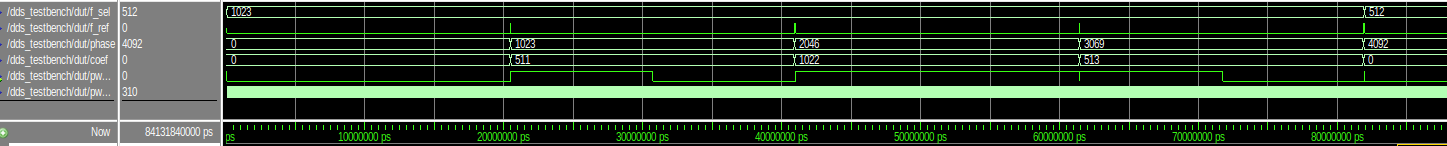
\includegraphics[width=\linewidth]{img/simulation_algo_uc1.png}
    \caption{Signalverläufe bei Use-Case \#1}
    \label{fig:sim_algo_uc1}
\end{figure}
\begin{figure}[h!]
    \centering
    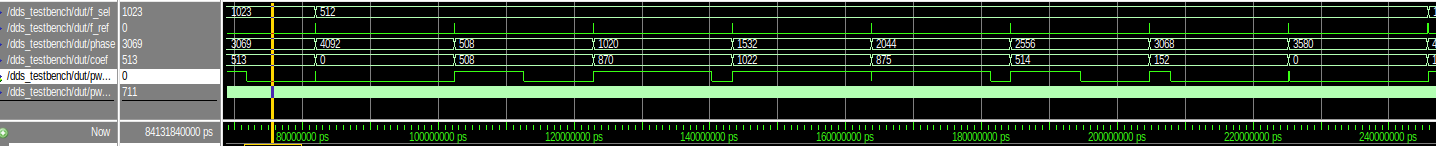
\includegraphics[width=\linewidth]{img/simulation_algo_uc2.png}
    \caption{Signalverläufe bei Use-Case \#2}
    \label{fig:sim_algo_uc2}
\end{figure}
\begin{figure}[h!]
    \centering
    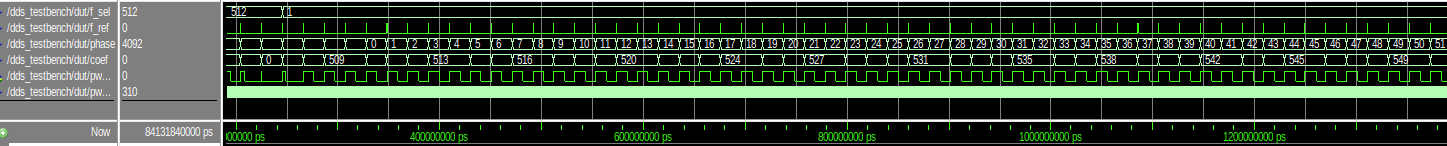
\includegraphics[width=\linewidth]{img/simulation_algo_uc3_1.png}
    \caption{Signalverläufe bei Use-Case \#3}
    \label{fig:sim_algo_uc3}
\end{figure}

\noindent Die Tests bestätigen, dass das System die vorgegebenen Frequenzen erzeugt und somit den funktionalen Anforderungen entspricht.
